\section{Exciton replicas and bosonic absorption}\label{sec:13.8}

Cold silicon begins to absorb light \SI{14.7}{meV} below the free-pair threshold $\Eg(0) + \omega_{\mathrm{TA}} = \SI{1.1875}{eV}$ of \cref{sec:13.5}. The electron and the hole that a photon creates together with a transverse acoustic phonon can stay bound, by $E_x^b = \SI{14.7}{meV}$ (\cref{sec:4.9,sec:6.5}). With the measured gap $\Eg(0) = \SI{1.1692}{eV}$ of \cref{sec:6.3} the bound threshold is $\Eg(0) + \omega_{\mathrm{TA}} - E_x^b = \SI{1.1728}{eV}$. Every phonon-assisted final state of this chapter has such a bound companion. In the rate of dark-matter scattering the companions are replicas of the exciton lines, one per phonon branch, which open below the free-pair onset of \cref{sec:13.1}. For a boson that is absorbed they matter more: between the indirect gap and the direct gap at \SI{3.4}{eV} absorption needs a phonon, and at \SI{1.2}{eV} the bound pairs carry most of it.

\subsection{Exciton--phonon coupling and the replica amplitude}

The Bethe--Salpeter equation of \cref{sec:4.9} at total crystal momentum $\vect{P}$ has the eigenstates
\begin{equation*}
  |\lambda(\vect{P})\rangle = \sum_{cv\vect{k}}A^\lambda_{cv\vect{k}}(\vect{P})\,c^\dagger_{c,\vect{k}+\vect{P}}c_{v\vect{k}}\,|0\rangle ,
\end{equation*}
with the hole at $\vect{k}$, the electron at $\vect{k}+\vect{P}$, and the energies $E_\lambda(\vect{P})$. They include the bound lines and the continuum, in which each free pair is dressed by the attraction. The density creates them from the ground state with $\langle\lambda|n_e(\vect{q})|0\rangle = \sqrt{g_{\mathrm{deg}}}\,\rho_{\lambda0}(\vect{q})$, the exciton form factor \cref{eq:10.5-formfactor}. The electron--phonon Hamiltonian \cref{eq:A.6-Hep} scatters the electron or the hole of an exciton, and it creates an exciton from the ground state. With the factor $N^{-1/2}$ and the phonon matrix element taken out, as for $g_{mn\nu}$, the matrix elements between the one-pair states above are
\begin{equation}
  \begin{aligned}
  g^x_{\lambda\lambda'\nu}(\vect{q},\vect{Q}) &= \sum_{cv\vect{k}}A^{\lambda*}_{cv\vect{k}}(\vect{q}+\vect{Q})\Bigl[\sum_{c'}g_{cc'\nu}(\vect{k}+\vect{q},\vect{Q})\,A^{\lambda'}_{c'v\vect{k}}(\vect{q}) - \sum_{v'}A^{\lambda'}_{cv',\vect{k}+\vect{Q}}(\vect{q})\,g_{v'v\nu}(\vect{k},\vect{Q})\Bigr] ,\\
  g^x_{\lambda0\nu}(\vect{Q}) &= \sum_{cv\vect{k}}A^{\lambda*}_{cv\vect{k}}(\vect{Q})\,g_{cv\nu}(\vect{k},\vect{Q}) ,
  \end{aligned}
  \label{eq:13.8-gx}
\end{equation}
for an exciton $\lambda'$ at $\vect{q}$ scattered into $\lambda$ at $\vect{q}+\vect{Q}$, and for an exciton created at $\vect{Q}$. The first is the exciton--phonon vertex of Antonius and Louie~\cite[Eq.~(49)]{antonius2022theory}: the phonon vertex of the electron, or of the hole, weighted by the envelopes of the two excitons. The hole term carries the minus sign that the reordering of fermion operators gave the hole paths in \cref{sec:13.2}. The density vertex between two excitons, from $\lambda'$ at $\vect{Q}$ to $\lambda$ at $\vect{q}+\vect{Q}$, has the same structure,
\begin{equation*}
  \rho_{\lambda\lambda'}(\vect{q}) = \sum_{cv\vect{k}}A^{\lambda*}_{cv\vect{k}}(\vect{q}+\vect{Q})\Bigl[\sum_{c'}\rho_{cc'}(\vect{k}+\vect{Q},\vect{q})\,A^{\lambda'}_{c'v\vect{k}}(\vect{Q}) - \sum_{v'}A^{\lambda'}_{cv',\vect{k}+\vect{q}}(\vect{Q})\,\rho_{v'v}(\vect{k},\vect{q})\Bigr] .
\end{equation*}

The second-order amplitude \cref{eq:13.2-T} is now evaluated with exciton states. The final state holds the exciton $\lambda$ at $\vect{q}+\vect{Q}$ and one phonon more in $(-\vect{Q},\nu)$ or one fewer in $(\vect{Q},\nu)$. With the density first, the intermediate exciton $\lambda'$ sits at $\vect{q}$ and the state holds the energy $\omega$. With the phonon first, it sits at $\vect{Q}$ and the phonon has already been emitted or absorbed:
\begin{keyresult}[Exciton--phonon replica amplitude]
\begin{equation}
  \begin{gathered}
  \langle f|n_e^{(2)}(\vect{q})|i\rangle = \sqrt{\frac{g_{\mathrm{deg}}}{N}}\,\bigl(n_{\vect{Q}\nu} + \tfrac12 \pm \tfrac12\bigr)^{1/2}M^\pm_{\lambda\nu}(\vect{q},\vect{Q}) , \\
  M^\pm_{\lambda\nu}(\vect{q},\vect{Q}) = \sum_{\lambda'}\left[\frac{g^x_{\lambda\lambda'\nu}(\vect{q},\vect{Q})\,\rho_{\lambda'0}(\vect{q})}{\omega - E_{\lambda'}(\vect{q})} + \frac{\rho_{\lambda\lambda'}(\vect{q})\,g^x_{\lambda'0\nu}(\vect{Q})}{-E_{\lambda'}(\vect{Q}) \mp \omega_{\vect{Q}\nu}}\right] ,
  \end{gathered}
  \label{eq:13.8-M}
\end{equation}
on the energy shell $\omega = E_\lambda(\vect{q}+\vect{Q}) \pm \omega_{\vect{Q}\nu}$, with $\lambda'$ running over every exciton state, bound or not, of every pair of bands. The phonon-assisted structure factor with excitonic final states is
\begin{equation}
  S^{\mathrm{PA}}(\vect{q},\omega) = \frac{2\pi g_{\mathrm{deg}}}{N\Vol}\sum_{\lambda\vect{Q}\nu\pm}\bigl(n_{\vect{Q}\nu} + \tfrac12 \pm \tfrac12\bigr)\,\bigl|M^\pm_{\lambda\nu}(\vect{q},\vect{Q})\bigr|^2\,\delta\bigl(E_\lambda(\vect{q}+\vect{Q}) \pm \omega_{\vect{Q}\nu} - \omega\bigr) ,
  \label{eq:13.8-S}
\end{equation}
which replaces \cref{eq:13.3-SPA} near the edge; it does not add to it.
\end{keyresult}
\noindent The spin enters once, through the singlet exciton created by the density or by the phonon; the scattering vertices conserve it. For a bound exciton $M^\pm_{\lambda\nu}$ grows as $\Vol^{1/2}$, as $\rho_{\lambda0}$ does (\cref{sec:10.5}), and $S^{\mathrm{PA}}$ is intensive.

Without the attraction, \cref{eq:13.8-M} is the amplitude of \cref{sec:13.2}. The exciton states are then single pairs, $A^\lambda_{cv\vect{k}} = 1$ for one pair and zero otherwise, and the exciton sums become band sums. The electron term of the first part is then path A of \cref{eq:13.2-paths} and its hole term path C; in the second part the electron term is path B and the hole term path D, each with its sign and its denominator. \Cref{eq:13.8-M} is the four-path amplitude written in exciton states, and on the energy shell the band-sum theorem of \cref{sec:13.2} turns it into \cref{eq:13.2-M}. The sum over final pairs $(c,v,\vect{k})$ then carries the factor $(2\pi/\Vol)\times2\times N^{-1}\sum_{\vect{k}\vect{Q}}$, and \cref{eq:13.8-S} becomes \cref{eq:13.3-SPA}. At $\vect{q} = 0$ the form factor $\rho_{\lambda'0}$ vanishes, and in $\rho_{\lambda\lambda'}(0)$ the electron and hole terms are both $\delta_{\lambda\lambda'}$ and cancel. The amplitude vanishes, as \cref{eq:13.2-q0} requires of any phonon-assisted density amplitude.

Screening enters as in \cref{sec:13.4}. The density vertex carries the external factor $1/\varepsilon_{\mathrm{mac}}(\vect{q},\omega)$, and the exchange interaction of the final pair at its momentum contains the pair channel. What \cref{eq:13.8-M} adds is the direct kernel, the electron--hole attraction of \cref{eq:4.9-bse}, in both the intermediate and the final states. That is the excitonic part of the ladder that \cref{sec:13.4} left out.

The vertices \cref{eq:13.8-gx} need the electron--phonon vertices and the exciton envelopes in one gauge: a Bloch state enters $g$ and $A^\lambda$ with the same phase, and a phase changed in one but not the other changes $|g^x|$. In practice the vertices come from Wannier interpolation in the gauge of the interpolated bands, and the Bethe--Salpeter equation is solved on the same states. It is needed at the momenta of the silicon pockets, with about $10^3$ points of $\vect{k}$ per pocket to resolve an exciton of radius $a_x = \SI{4.2}{nm}$. For silicon and germanium that calculation is open, and a converged replica spectrum from it is the open problem of this section.

\subsection{Completeness and the two-pair test}

The sums over $\lambda'$ in \cref{eq:13.8-M} run over every one-pair state at $\vect{q}$ and at $\vect{Q}$, including the pairs whose hole lies deep in the valence band, which the hole terms of $g^x$ and $\rho_{\lambda\lambda'}$ reach. Dropping those hole terms is the exciton version of truncating the band sum to empty bands, which cost a factor of 2.4 in the model of \cref{we:13-exchange}, with the phase of its displacement wave at the cell origin. A Bethe--Salpeter basis of a few bands on each side of the gap describes the final exciton well, but not the intermediate ones, which reach every band. The $f$-sum test of the density vertices applies to the intermediate sums here as it does to \cref{eq:13.2-M}.

The space of one pair must also be the whole space of intermediate states. For independent electrons every intermediate state of \cref{eq:13.2-T} holds exactly one pair, because each vertex moves one electron (\cref{sec:13.2}). With the electron--hole interaction this is no longer exact. The Coulomb interaction contains terms that create a pair while they scatter an electron or a hole, so an exact eigenstate with one pair carries an admixture of states with two pairs, and the exact ground state an admixture of virtual pairs. \Cref{eq:13.8-M} keeps the Tamm--Dancoff space of one pair for both the intermediate and the final excitons. It is complete if the states with two pairs add nothing beyond the one-pair terms. Without interaction they do not exist, and the formula reduces to the four paths exactly. With the interaction it is unproven, and the completeness of the replica expansion reduces to the size of the two-pair sector. Its parametric estimate is the ratio of the binding energy to the gap, $E_x^b/\Eg \approx \SI{1}{\percent}$ in silicon, an estimate and not a bound.

A model with an exact two-pair sector would size this correction: a two-band chain of 8 to 12 cells with a contact attraction between electron and hole and one phonon mode, diagonalized with its states of zero, one and two pairs and compared with \cref{eq:13.8-M} built from its exact one-pair excitons.

\subsection{Replicas near the silicon edge}

Near the edge the final exciton lies within a few $E_x^b$ of the band extrema, while every intermediate exciton is far from the energy shell. By \cref{eq:13.2-doff} the distance is at least \SI{0.7}{eV} at the onset of \cref{we:13-onset}, and \SI{1.11}{eV} for absorption between the indirect and the direct gap. This separation of scales leads to a closed form. The vertices $g^x_{\lambda\lambda'\nu}$ and $\rho_{\lambda\lambda'}$ are linear in the final envelope $A^{\lambda*}(\vect{q}+\vect{Q})$, so that
\begin{equation*}
  M^\pm_{\lambda\nu}(\vect{q},\vect{Q}) = \sum_{\vect{k}}A^{\lambda*}_{cv\vect{k}}(\vect{q}+\vect{Q})\,M^{x\pm}_{cv\nu}(\vect{k},\vect{q},\vect{Q}) ,
\end{equation*}
where $M^{x\pm}$ is the amplitude into the free final pair $(c,\vect{k}+\vect{q}+\vect{Q};\,v,\vect{k})$ with exciton intermediate states. The final pair enters $M^{x\pm}$ also through the energy $\omega$ in the denominators, which moves by at most $E_x^b$ between a bound and a free final pair, a relative change $E_x^b/\delta_{\mathrm{off}}$ of about \SI{2}{\percent} at the onset and less in absorption. With free intermediate pairs, $M^{x\pm}$ is the $M^\pm$ of \cref{eq:13.2-M}. The attraction among the intermediate pairs changes it, as it changes the optical spectrum of silicon near its main peak (\cref{sec:4.9}). It does so smoothly across the zone, and changes the size of $M^{x\pm}$ at the extrema, not its variation over the small region of $\vect{k}$ that the envelope covers. With $M^{x\pm}$ held at its value $M^x_\nu$ at the extrema and $\sum_{\vect{k}}A^{\lambda*}_{\vect{k}} = \Vol^{1/2}F^*_\lambda(0)$ (\cref{sec:4.9}),
\begin{equation}
  M^\pm_{\lambda\nu}(\vect{q},\vect{Q}) \simeq \Vol^{1/2}\,F^*_\lambda(0)\,M^x_\nu ,
  \label{eq:13.8-elliott}
\end{equation}
the Elliott form \cref{eq:4.9-elliott} with the phonon-assisted amplitude in place of the density vertex~\cite{elliott1957intensity}. Only $s$ states contribute, and the shape of the edge is fixed by the final pair alone.

The final excitons are labeled by their relative motion, a bound level $n$ or a continuum state, and by their total momentum $\vect{P} = \vect{q}+\vect{Q}$, with energy $\Eg + E^{\mathrm{rel}} + (\vect{P} - \vect{k}_{\mathrm{c}})^2/2M_{\mathrm{eh}}$ near a valley by \cref{eq:4.9-dispersion}, where $M_{\mathrm{eh}}$ is the translational mass of the pair (\cref{sec:13.1}), taken isotropic. The sum over $\vect{Q}$ in \cref{eq:13.8-S} is a sum over $\vect{P}$. Insert \cref{eq:13.8-elliott} and take $T \to 0$, so that only emission survives. The factors combine as $(2\pi g_{\mathrm{deg}}/N\Vol)\,\Vol\sum_{\vect{P}} = (4\pi/N)\,N\Omega\int\dd^3\kappa/(2\pi)^3 = 4\pi\Omega\int\dd^3\kappa/(2\pi)^3$, with $\vect{\kappa} = \vect{P} - \vect{k}_{\mathrm{c}}$. The sum of $|F_\lambda(0)|^2$ over the relative states at fixed $E^{\mathrm{rel}} = E$ is the bracket of \cref{eq:10.5-lines}, which we write $\mathcal{W}_x(E)$: lines $\delta(E + E_x^b/n^2)/(\pi a_x^3n^3)$ below zero and the continuum $(2\mu_x)^{3/2}E^{1/2}F_{\mathrm{Fermi}}/4\pi^2$ above, with the Fermi factor \cref{eq:2.2-fermi} at $\xi_{\mathrm{C}} = (E_x^b/E)^{1/2}$. The integral over $\vect{\kappa}$ is the density of states of the center-of-mass motion, which the phonon leaves free. Per valley, branch and hole band,
\begin{equation*}
  S^{\mathrm{PA}}(\vect{q},\omega) \simeq 4\pi\Omega\,|M^x_\nu|^2\int\dd E\;\mathcal{W}_x(E)\,\frac{(2M_{\mathrm{eh}})^{3/2}(x - E)^{1/2}}{4\pi^2} , \qquad x = \omega - E_{\mathrm{min}}^{\mathrm{PA}}(\vect{q}) ,
\end{equation*}
with $E_{\mathrm{min}}^{\mathrm{PA}}(\vect{q})$ the free-pair threshold of \cref{eq:13.1-EPA}. Without the attraction, $\mathcal{W}_x$ is the free continuum alone, $\int_0^x\dd E\,E^{1/2}(x - E)^{1/2} = \pi x^2/8$, and the result is $\Omega(\mu_xM_{\mathrm{eh}})^{3/2}|M_\nu|^2x^2/4\pi^2$. That is \cref{eq:13.3-near}, because $\mu_xM_{\mathrm{eh}}$ is the product of the electron and hole masses for parabolic bands. Divided by this free-pair edge, the masses cancel. With $(2\mu_x)^{3/2} = 1/[a_x^3(E_x^b)^{3/2}]$ from \cref{eq:4.9-WM}, each line weight $1/(\pi a_x^3n^3)$ is $4\pi(E_x^b)^{3/2}/n^3$ in units of the continuum coefficient. Normalizing by $\pi x^2/8$ then gives the edge in closed form.
\begin{keyresult}[Replica edge in the Wannier--Mott limit]
Near the threshold of one branch, at fixed $\vect{q}$ and $T \to 0$, a phonon-assisted spectrum whose free-pair form is $A_\nu x^2$ becomes, with excitonic final states,
\begin{equation}
  A_\nu\biggl[32\,(E_x^b)^{3/2}\sum_{n\ge1}\frac{(x + E_x^b/n^2)^{1/2}}{n^3} + \frac{8}{\pi}\int_0^x\dd E\;E^{1/2}(x - E)^{1/2}\,\frac{2\pi\xi_{\mathrm{C}}}{1 - \ee^{-2\pi\xi_{\mathrm{C}}}}\biggr] ,
  \label{eq:13.8-edge}
\end{equation}
with $\xi_{\mathrm{C}} = (E_x^b/E)^{1/2}$ and each line term counted for $x > -E_x^b/n^2$. The coefficient $A_\nu$ is the one of \cref{eq:13.3-near} for dark-matter scattering and of \cref{eq:6.5-edge} for light.
\end{keyresult}
\noindent Each bound level becomes a replica edge that opens at $E_{\mathrm{min}}^{\mathrm{PA}}(\vect{q}) - E_x^b/n^2$ and rises as a square root: a line of the relative motion, spread by the center-of-mass motion. The continuum starts from zero at the free-pair threshold, but as $(32/3)(E_x^b)^{1/2}x^{3/2}$ instead of $x^2$, since the Fermi factor makes its relative-motion weight finite at the edge. These are the exponents that \cref{sec:13.3} anticipated: $\frac12$ for a replica and $\frac32$ for the excitonic continuum at fixed $\vect{q}$, and one power more each after the average over the directions of $\vect{q}$ (\cref{eq:13.3-pon}). The strength follows from the ratio of the $1s$ term to the free one at equal distance $x$ from their own thresholds, $32(E_x^b/x)^{3/2}$: 32 at $x = E_x^b$ and 5.1 at \SI{50}{meV}. The weight of the relative motion is redistributed as in \cref{sec:10.5}: the lines together hold what the free pairs hold within $8.0\,E_x^b$ of the edge, and the Fermi factor keeps the continuum above its free value far beyond.

\begin{figure}[tbp]
  \centering
  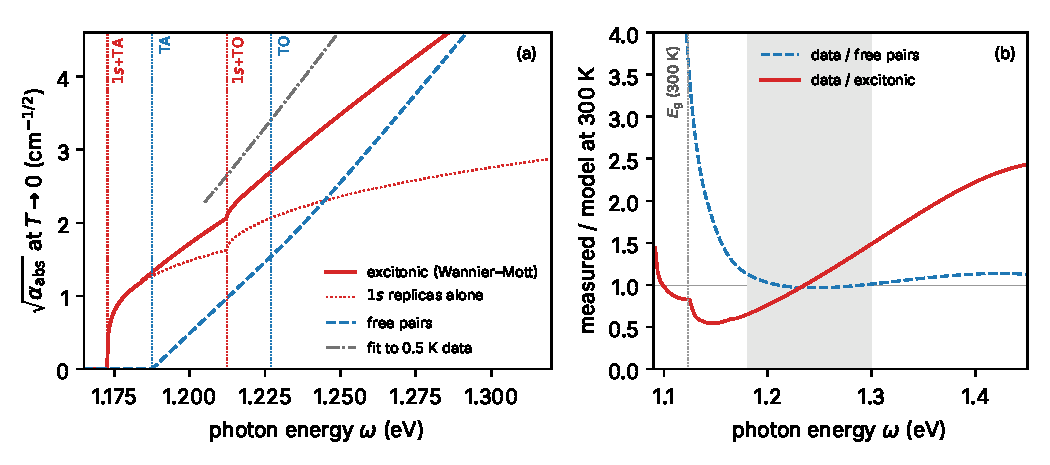
\includegraphics[width=\linewidth]{figures/ch13/fig13_8.pdf}
  \caption{Phonon-assisted absorption edge of silicon with excitonic final states. (a) $\sqrt{\alpha_{\mathrm{abs}}}$ at $T \to 0$ against the photon energy. Red: \cref{eq:13.8-edge} for the transverse acoustic and transverse optical branches, $\omega_{\mathrm{TA}} = \SI{18.27}{meV}$ and $\omega_{\mathrm{TO}} = \SI{57.73}{meV}$, with weights $5.5:4.0$~\cite{rajkanan1979absorption,stanford2021photoelectric}, $\Eg(0) = \SI{1.1692}{eV}$ and $E_x^b = \SI{14.7}{meV}$ for both hole bands; dotted, the two $1s$ replicas alone. Blue, dashed: the free-pair edge of \cref{sec:13.5}. Each model has one scale, fitted as in \cref{sec:13.5} to the measured \SI{300}{K} absorption between 1.18 and \SI{1.30}{eV}~\cite{franta2017temperature}. Gray, dash-dotted: the free-pair form fitted to measurements between 0.5 and \SI{295}{K}, with an effective gap of \SI{1.134}{eV}, evaluated at \SI{0.5}{K} and drawn above \SI{1.205}{eV}, the lowest photon energy measured~\cite[Eqs.~(4)--(7)]{stanford2021photoelectric}. Vertical lines: the $1s$ replica thresholds $\Eg - E_x^b + \omega_\nu$ (red) and the free-pair thresholds $\Eg + \omega_\nu$ (blue). (b) Measured absorption at \SI{300}{K} divided by each model at \SI{300}{K}, both branches with their phonon occupations; gray band, the fitted interval. Effective-mass models with constant matrix elements, not calculations.}
  \label{fig:13-replicas}
\end{figure}

\Cref{fig:13-replicas}a shows \cref{eq:13.8-edge} for cold silicon. The $1s$ replica of the transverse acoustic branch opens at \SI{1.1728}{eV} and the $2s$ replica at \SI{1.1838}{eV}, both below the free-pair threshold at \SI{1.1875}{eV}; the transverse optical replica opens at \SI{1.2122}{eV}. With the same $|M^x_\nu|^2$ the excitonic edge of the two branches exceeds the free-pair one by a factor of 81 at \SI{1.200}{eV}, 16 at \SI{50}{meV} above the free threshold and 7.3 at \SI{100}{meV}, and at \SI{1.200}{eV} the $1s$ replica holds three quarters of it.

The measured spectra test the shape. Fitted in the same interval of the \SI{300}{K} data, the excitonic form needs a scale 0.154 times that of the free-pair form, since the Fermi factor already supplies part of the absorption there. Neither form follows the data over the whole range (\cref{fig:13-replicas}b). The free-pair form falls short within \SI{40}{meV} of the gap, by the factor 2.0 at \SI{17}{meV} found in \cref{sec:13.5}. The hydrogenic form overshoots there by up to 1.8 and falls short by 1.5 to 2.5 between 1.3 and \SI{1.6}{eV}, where the parabolic bands and the hydrogenic continuum of \cref{sec:10.5} no longer hold. The edge region is where the excitonic form belongs, and there the measurements at low temperature are the test. At \SI{1.21}{eV}, the lowest energy measured at \SI{0.5}{K}, the fit to the measurements, evaluated at that temperature, is \SI{6.4}{cm^{-1}}, the excitonic form 4.0 and the free-pair form \SI{0.77}{cm^{-1}}. With the decrease of the branch strength between the lowest temperature and \SI{295}{K} found in \cref{sec:13.5}, a factor 0.61, the excitonic value becomes 6.6 and the free-pair one 1.3. The fit itself needs an effective gap of \SI{1.134}{eV}, \SI{35}{meV} below the true one: a free-pair form can follow an excitonic edge only by moving its threshold down.

For dark-matter scattering the same construction applies at each $\vect{q}$, with $A_\nu$ the coefficient of \cref{eq:13.3-near} and the thresholds $E_{\mathrm{min}}^{\mathrm{PA}}(\vect{q}) - E_x^b/n^2$. The binding energy is that of the pair at the momentum $\vect{q}+\vect{Q}^*$, near $\vect{k}_{\mathrm{c}}$, where the hole sits near the valence maximum and the measured \SI{14.7}{meV} applies; its variation along the dispersion of the pair is \cref{eq:E.15-disp}. The lightest mass at which the $1s$ replica opens follows from \cref{eq:13.1-mPA} with $\Eg$ replaced by $\Eg - E_x^b$, as \cref{sec:13.1} found, and its value and status belong to \cref{sec:13.9}.

\subsection{Phonon-assisted absorption of bosonic dark matter}

Absorption of a boson probes the response at $\vect{q} = \vect{p}_\phi$, about $10^{-3}m_\phi$, and $\omega = m_\phi$ (\cref{eq:8.2-abs}). In silicon between the excitonic edge at \SI{1.1728}{eV} and the direct gap $E_{\mathrm{dir}} = \SI{3.4}{eV}$ no vertical pair exists. Every first-order transition at $\vect{q} \simeq 0$ is then off the energy shell, and the window of \cref{eq:13.6-window}, with the vertical gap as the zero-phonon edge, extends to $E_{\mathrm{dir}} - \delta_{\mathrm{w}} = \SI{3.1}{eV}$. Inside it every response row is phonon-assisted. Its structure factor is \cref{eq:13.3-SPA} at $\vect{q} = 0$ with the vertices of the two rows in place of $\rho$, or \cref{eq:13.8-S} near the edge. Each of the three rates of \cref{sec:10.7} therefore holds there with its response replaced by the phonon-assisted one. The bosons differ in whether that response is measured.

The dark photon has no phonon-assisted amplitude of its own at first order in $g$. It couples to the electromagnetic current of electrons and nuclei with $\zeta$ times the charge of the photon, and every second-order amplitude into a pair and one phonon reduces to that of light or vanishes. The electron current with one electron--phonon vertex is the amplitude of light, \cref{eq:6.5-M} with the velocity vertex, and its square summed over final states is the measured $\varepsilon_2^{\mathrm{PA}}$. The longitudinal polarization couples to the charge density at $\vect{q} = \vect{p}_\phi$, and the phonon-assisted density amplitude there is, by continuity, $(q/\omega)$ times the velocity amplitude (\cref{eq:13.5-Mlim}). It is the same amplitude written another way, and adding the density form of \cref{sec:13.2} to the current form would count the transition twice. The nuclear current, finally, changes a phonon occupation at $\vect{Q} \simeq \vect{p}_\phi$ without moving an electron, while the electron--phonon vertex moves one electron and changes one occupation. Together they either leave two occupations changed, a final state with two phonons, or remove the phonon the current created and leave a vertical pair, which needs $\omega \ge E_{\mathrm{dir}}$; in silicon the Born charges vanish in any case. The rate is \cref{eq:10.7-dp} with $L = \varepsilon_2^{\mathrm{PA}}/(\varepsilon_1^0)^2$ at the temperature of the detector (\cref{sec:13.4,sec:13.5}). At the edge $\varepsilon_2^{\mathrm{PA}}$ is of order $10^{-4}$, so the phonon-assisted part of the photon self-energy does nothing to the mixing, and $\zeta_{\mathrm{eff}} = \zeta/\varepsilon_1^0$. What the dark photon needs is the measured edge itself, brought to millikelvin temperatures and resolved into its excitonic structure, as \cref{we:13-darkphoton-edge} shows.

The axion-like particle couples through the spin current $\mathcal{J}_e$ (\cref{sec:10.7-alp}). The electron--phonon vertex is diagonal in spin. The spin structure of the phonon-assisted amplitude is therefore that of the one spin operator in $\mathcal{J}_e$, and the spin trace of \cref{sec:10.7-alp} goes through unchanged: $S^{\mathrm{PA}}_{\mathcal{J}\mathcal{J}} = \frac34S^{\mathrm{PA}}_{jj}$ and $\varGamma = (3m_\phi^2/4m_e^2)(g_{aee}^2/e^2)\,\sigma_1^{\mathrm{PA}}$, with $\sigma_1^{\mathrm{PA}} = m_\phi\varepsilon_2^{\mathrm{PA}}$, for independent electrons without spin--orbit coupling. At equal couplings it is $(3m_\phi^2/4m_e^2e^2)|\varepsilon|^2 = 7.3\times10^{-9}$ of the dark-photon rate at \SI{1.2}{eV}. The caveats of \cref{sec:10.7-alp} take a specific form at the edge. The spin current creates triplet pairs, which feel the direct kernel and not the exchange one (\cref{eq:10.5-triplet}). The replica lines are therefore the same as in the measured singlet edge, up to the exchange splitting, which is about $2\times10^{-3}$ of the binding (\cref{sec:10.5}). The pair channel of \cref{sec:13.4}, a Coulomb screening at the pair momentum, is absent from the triplet response, and its size is not known for the singlet either.

The scalar couples through two rows, the density and the kinetic energy (\cref{sec:10.7-scalar}). The phonon-assisted density amplitude vanishes at $\vect{q} = 0$ by \cref{eq:13.2-q0}, so the density row enters at order $p_\phi$ and its rate at order $v^2$. The kinetic row, however, does not vanish. Its phonon-assisted amplitude $M^\pm_{\mathcal{T},cv\nu}(\vect{k},\vect{Q})$ is \cref{eq:13.2-M} at $\vect{q} = 0$ with the vertical kinetic elements $(\mathcal{T}_e)_{mn}(\vect{k}) = \langle m\vect{k}|p^2/2m_e|n\vect{k}\rangle$ in place of $\rho_{mn}$, and its intraband terms no longer cancel. Path A with $p = v$ and path B with $p = c$ add to $g_{cv\nu}(\vect{k},\vect{Q})[(\mathcal{T}_e)_{vv}(\vect{k}) - (\mathcal{T}_e)_{cc}(\vect{k}+\vect{Q})]/\omega$, the difference of the kinetic energies of the two band states, where the density has $\rho_{vv} = \rho_{cc} = 1$. The whole amplitude has a compact form. In the operator form of \cref{eq:13.2-M} (\cref{app:D.35}), $\langle c|y\,(\varepsilon_v + \omega - h)^{-1}x + x\,(\varepsilon_v \mp \omega_{\vect{Q}\nu} - h)^{-1}y|v\rangle$ with $x = p^2/2m_e$ and $y$ the phonon vertex, write $x = h - V$, with $h$ the one-electron Hamiltonian and $V$ everything in it but the kinetic energy. The part $h$ acts on $|v\rangle$ in the first term and on $\langle c|$ in the second, where it returns $\varepsilon_v$ and $\varepsilon_c$, and the resolvents return $1/\omega$ and $-1/\omega$ on the shell. With $\varepsilon_c - \varepsilon_v = \omega \mp \omega_{\vect{Q}\nu}$,
\begin{equation}
  M^\pm_{\mathcal{T},cv\nu}(\vect{k},\vect{Q}) = -\Bigl(1 \mp \frac{\omega_{\vect{Q}\nu}}{\omega}\Bigr)\,g_{cv\nu}(\vect{k},\vect{Q}) - M^\pm_{V,cv\nu}(\vect{k},\vect{Q}) ,
  \label{eq:13.8-MT}
\end{equation}
where $M^\pm_V$ is \cref{eq:13.2-M} at $\vect{q} = 0$ with the matrix elements of $V$ in place of $\rho$. The first term is the electron--phonon vertex itself. The second is the phonon-assisted amplitude of the crystal potential, the counterpart of $\langle c|p^2/2m_e|v\rangle = -\langle c|V|v\rangle$ of \cref{sec:10.7-scalar}, and like it weighted toward the cores. Both are of order $g$ in energy units, and nothing cancels them. \Cref{eq:10.7-scalar} with the phonon-assisted response is
\begin{equation}
  \begin{gathered}
  \varGamma = \frac{g_{\phi ee}^2}{2\,m_\phi m_e^2}\,S^{\mathrm{PA}}_{\mathcal{T}\mathcal{T}}(0,m_\phi) , \\
  S^{\mathrm{PA}}_{\mathcal{T}\mathcal{T}}(0,\omega) = \frac{4\pi}{\Omega}\Bigl\langle\!\Bigl\langle\sum_{\nu cv\pm}\bigl(n_{\vect{Q}\nu} + \tfrac12 \pm \tfrac12\bigr)\bigl|M^\pm_{\mathcal{T},cv\nu}\bigr|^2\delta\bigl(\varepsilon_{c,\vect{k}+\vect{Q}} - \varepsilon_{v\vect{k}} \pm \omega_{\vect{Q}\nu} - \omega\bigr)\Bigr\rangle\!\Bigr\rangle ,
  \end{gathered}
  \label{eq:13.8-scalar}
\end{equation}
unscreened, for a point group without a polar vector, inside the window; near the edge the final pairs are the excitons of \cref{eq:13.8-S} with the kinetic row in place of the density. No measurement provides this response, and it is not proportional to $\varepsilon_2^{\mathrm{PA}}$, since \cref{eq:13.8-MT} has no velocity vertex in it. The comparison with the axion-like particle in \cref{sec:10.7-scalar} carries over. The kinetic amplitude is of the order of the vertex $g$, while the axion-like amplitude carries $m_\phi/m_e$ times an electron velocity. At equal couplings the scalar is therefore absorbed far more strongly, by a factor that only a calculation fixes. The phonon-assisted kinetic absorption has been computed for the intraband transitions of a superconducting metal~\cite[Sect.~V, Eq.~(72)]{mitridate2021dark}; a silicon rate built from vertical transitions has below about \SI{3}{eV} only the tails of the smearing~\cite[Sect.~IV]{mitridate2021dark}. The interband channel of \cref{eq:13.8-MT,eq:13.8-scalar} at the indirect edge of an insulator needs, for its evaluation, a phonon-assisted kinetic row with all-electron kinetic matrix elements.

\begin{workedexample}{A dark photon of 1.2 eV in cold silicon}\label{we:13-darkphoton-edge}
At $m_\phi = \SI{1.200}{eV}$ a dark photon sits \SI{12.5}{meV} above the free-pair threshold $\Eg(0) + \omega_{\mathrm{TA}} = \SI{1.1875}{eV}$ and \SI{27.2}{meV} above the $1s$ replica, below both transverse optical thresholds. Only the transverse acoustic branch absorbs, by emission.

\emph{Cold absorption.} Stanford and co-workers fitted their data at 0.5 to \SI{295}{K} with the free-pair form $\alpha_{\mathrm{abs}} = \sum_\nu C_\nu c_0(\omega - E_{\mathrm{g}1} - \omega_\nu)^2$ at low temperature, with the branch weights $C_{\mathrm{TA}} = 5.5$ and $C_{\mathrm{TO}} = 4.0$, the strength $c_0 = \SI{325}{eV^{-2}.cm^{-1}}$ and an effective gap $E_{\mathrm{g}1} = \SI{1.134}{eV}$~\cite[Eqs.~(4)--(7)]{stanford2021photoelectric}. Evaluated at \SI{0.5}{K}, it gives $\alpha_{\mathrm{abs}} = 5.5\times\SI{325}{eV^{-2}.cm^{-1}}\times(\SI{0.0477}{eV})^2 = \SI{4.07}{cm^{-1}}$ from its transverse acoustic term and \SI{0.09}{cm^{-1}} from the transverse optical one, which its lowered gap opens: \SI{4.16}{cm^{-1}}, \SI{6}{meV} below their lowest photon energy. The \SI{20}{K} data of Macfarlane and co-workers~\cite{macfarlane1958fine} give \SI{0.21}{cm^{-1}} at this energy, twenty times less; near the edge the cold datasets differ by that much (\cref{sec:13.9-rates}). The excitonic edge of \cref{fig:13-replicas} reaches \SI{2.95}{cm^{-1}} (4.8 with the strength factor 0.61), the free-pair edge transferred to millikelvin temperatures in \cref{sec:13.5} only \SI{0.24}{cm^{-1}}, and the \SI{300}{K} data used without transfer \SI{27.3}{cm^{-1}}.

\emph{Loss function.} With the fit value $\alpha_{\mathrm{abs}} = \SI{4.16}{cm^{-1}}$, $n_r = 3.565$ from the \SI{300}{K} data and $\hbar c/\omega = \SI{1.644e-5}{cm}$,
\begin{equation*}
  \varepsilon_2^{\mathrm{PA}} = n_r\,\alpha_{\mathrm{abs}}\,\frac{\hbar c}{\omega} = 2.44\times10^{-4} , \qquad
  L = \frac{\varepsilon_2^{\mathrm{PA}}}{(\varepsilon_1^0)^2} = \frac{2.44\times10^{-4}}{12.71^2} = 1.51\times10^{-6} .
\end{equation*}
The medium suppresses the rate by $|\varepsilon|^2 = 161.5$ against the vacuum mixing.

\emph{Rate.} With $\rho_\chi = \SI{0.3}{GeV.cm^{-3}}$ and $\rho_T = \SI{2.33}{g.cm^{-3}}$, $(\rho_\chi/\rho_T)/\hbar = 6.17\times10^{33}$ per kilogram-year, as in \cref{we:10-darkphoton}, and \cref{eq:10.7-dp} gives
\begin{equation*}
  \mathcal{R} = 6.17\times10^{33}\times1.51\times10^{-6}\,\zeta^2 = 9.3\times10^{27}\,\zeta^2\ \text{per kilogram-year} .
\end{equation*}
Three events in a kilogram-year need $\zeta = 1.8\times10^{-14}$. The untransferred \SI{300}{K} data would claim a rate 6.6 times larger and $\zeta = 7.0\times10^{-15}$; the transferred free-pair edge a rate 17 times smaller and $\zeta = 7.5\times10^{-14}$, and the \SI{20}{K} data a rate 20 times smaller. At \SI{1.2}{eV} the correction that matters is the bound pair: in the excitonic edge three quarters of the absorption at this energy is the $1s$ replica, which neither the warm data nor the free-pair transfer represents.
\end{workedexample}
